% !TEX program = lualatex
\documentclass[a4paper,10pt,oneside,openany]{ltjsreport}
\usepackage[margin=21mm,top=19mm,bottom=20mm]{geometry}
\usepackage[haranoaji]{luatexja-preset}
\usepackage{amsmath,amssymb,graphicx,booktabs,longtable,xcolor,float}
\usepackage[unicode,colorlinks=true,linkcolor=blue!45!black,urlcolor=blue!45!black]{hyperref}
\usepackage{caption}
\captionsetup{font=small,labelfont=bf}
\setcounter{tocdepth}{0}
\setlength{\parskip}{0.45em}
\setlength{\parindent}{1em}
\raggedbottom
\newcommand{\sourcefile}[1]{{\small\texttt{\detokenize{#1}}}}
\begin{document}


\title{\Huge 実験1\\[0.6em]\LARGE 非相互作用系による検算\\[1em]\large 一次元HubbardモデルのUHF計算}

\author{保存結果の解析レポート}\date{2026年11月2日}\maketitle

\chapter*{概要}

相互作用を除いた $U=0$ の半充填系を用いて、粒子数、エネルギー、スピン対称性を検算する。両境界条件とも1反復で収束した。$E_{\rm int}=0$ であり、全エネルギーは運動エネルギーと一致する。本実験で変えたのは境界条件だけであり、$U$ や粒子数に関する掃引は行っていない。

対象は2ケース、保存図9枚である。収束は2ケース、未収束は0ケース。本書では生成物の種類ごとに章を設け、同じ条件のOBCとPBCを並べて読む。

\tableofcontents

\chapter{計算ログ：条件と最終結果}

\sourcefile{uhf_results.txt}

\section*{計算条件と量の定義}

$L=50$、$t=1$、温度 $T=0$、外部電場なし。全エネルギーと軌道エネルギーは $t$ を単位とする。
OBCは開放端、PBCはサイト50と1も接続する周期境界である。$N_e=N_\uparrow+N_\downarrow$、$\Delta N=N_\uparrow-N_\downarrow$ と定義する。
収束判定は混合前の密度残差 $r<10^{-10}$、最大反復回数は10000である。
表の「未」は未収束の最終再評価値であり、その桁数は精度保証ではない。

\begin{center}\small\setlength{\tabcolsep}{4pt}
\begin{longtable}{lrrrr}
\toprule
条件 & $N_e$ & $\Delta N$ & $U/t$ & mixing \\ \midrule
\endhead
基準 & 50 & 0 & 0 & 0.25 \\
\bottomrule\end{longtable}\end{center}

\section*{最終エネルギー}

$E=E_{\rm kin}+E_{\rm int}$、$E_{\rm int}=U\sum_i n_{i\uparrow}n_{i\downarrow}$。全エネルギーは占有軌道固有値の単純な総和ではなく、平均場の二重計数を除いた量である。

\begin{center}\small\setlength{\tabcolsep}{4pt}
\begin{longtable}{lrrrr}
\toprule
条件/境界 & 状態 & $E$ & $E_{\rm kin}$ & $E_{\rm int}$ \\ \midrule
\endhead
OBC & 収束 & -62.945484561 & -62.945484561 & 0.000000000 \\
PBC & 収束 & -63.703884440 & -63.703884440 & 0.000000000 \\
\bottomrule\end{longtable}\end{center}

相互作用を除いた $U=0$ の半充填系を用いて、粒子数、エネルギー、スピン対称性を検算する。両境界条件とも1反復で収束した。$E_{\rm int}=0$ であり、全エネルギーは運動エネルギーと一致する。本実験で変えたのは境界条件だけであり、$U$ や粒子数に関する掃引は行っていない。

\section*{原資料と再利用}

出典は \sourcefile{results_vault/experiment_01/} 内の各条件/OBC・PBCのログ、CSV、PNG。\\ 補助資料は \sourcefile{experiment_conditions.md} と \sourcefile{uhf.jl}。値は保存済みの結果から採り、SCFを再実行していない。

条件名は原資料のディレクトリ名である。本実験は新規計算の結果のみである。

再利用データは独立した追加試行ではない。本書の解釈は保存された有限サイズ・UHF解の範囲に限る。

\chapter{密度CSV：電荷分布と二重占有}

\sourcefile{density_checkpoint.csv}

CSVの50サイトすべてから $q_i=n_{i\uparrow}+n_{i\downarrow}$、$m_i=n_{i\uparrow}-n_{i\downarrow}$、
$D=L^{-1}\sum_i n_{i\uparrow}n_{i\downarrow}$ を計算した。密度の各スピン成分は0以上1以下で、総和は指定した粒子数に一致することを確認した。未収束時のCSVは最後の混合密度を対角化して得た出力密度であり、固定点の密度とは限らない。

\begin{center}\small\setlength{\tabcolsep}{4pt}
\begin{longtable}{lrrrr}
\toprule
条件/境界 & 状態 & $\min q_i$ & $\max q_i$ & $D$ \\ \midrule
\endhead
OBC & 収束 & 1.000000 & 1.000000 & 0.250000 \\
PBC & 収束 & 1.000000 & 1.000000 & 0.250000 \\
\bottomrule\end{longtable}\end{center}

両境界条件とも各サイトで $n_{i\uparrow}=n_{i\downarrow}=0.5$、$q_i=1$ である。開放端があっても、この半充填・非相互作用の条件では電荷密度の端での変調は現れない。総粒子数は50で、境界条件を変えても保存される。

\chapter{SCFエネルギー：反復による変化}

\sourcefile{scf_energy.png}

初期の一様密度がすでに自己無撞着なので、エネルギー履歴は各1点である。PBCではOBCより $0.758399879117$ 低い。これは密度変化を伴わず、閉じた鎖と開いた鎖の固有値の違いだけで生じる。

各図の横軸は反復回数、縦軸は各反復で評価した全エネルギーである。図ごとに軸範囲が異なるため、見かけの傾きだけを比較しない。最終ログ値は反復終了後の再評価であり、履歴の最終点とわずかに異なる場合がある。

\begin{center}\small\setlength{\tabcolsep}{4pt}
\begin{longtable}{lrrr}
\toprule
条件/境界 & 初回 $E$ & 最終 $E$ & 最後の履歴の $|\Delta E|$ \\ \midrule
\endhead
OBC & -62.945485 & -62.945485 & 履歴1点 \\
PBC & -63.703884 & -63.703884 & 履歴1点 \\
\bottomrule\end{longtable}\end{center}

\begin{figure}[H]\centering

\begin{minipage}{0.49\linewidth}\centering

\textbf{OBC：収束}\par

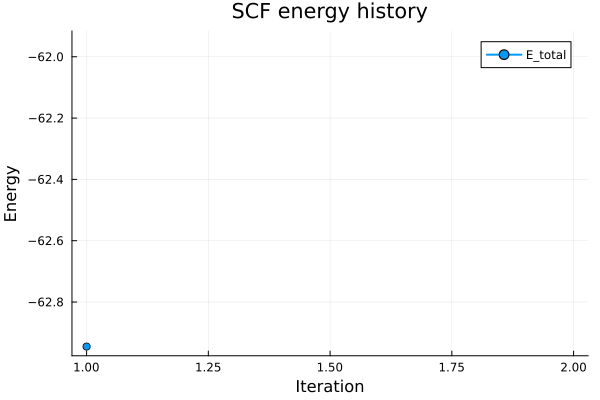
\includegraphics[width=\linewidth]{../../results_vault/experiment_01/OBC/scf_energy.png}

\end{minipage}\hfill%
\begin{minipage}{0.49\linewidth}\centering

\textbf{PBC：収束}\par

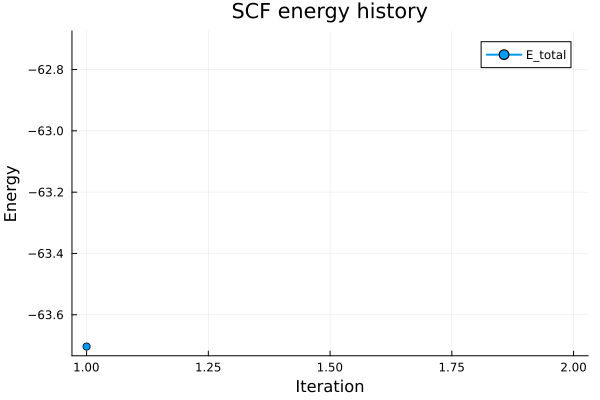
\includegraphics[width=\linewidth]{../../results_vault/experiment_01/PBC/scf_energy.png}

\end{minipage}

\caption{基準条件。SCFエネルギーの比較。左：OBC、右：PBC。}\end{figure}

\chapter{SCF残差：自己無撞着性}

\sourcefile{scf_residual.png}

最終再評価の残差は両方ともログ上で0である。対数軸に厳密な0は表示できないため、保存図に見える有限位置の点を残差の数値として読んではならない。1点だけの履歴から収束速度の比較はできない。

残差は $r=\max_{i,\sigma}|F[n]_{i\sigma}-n_{i\sigma}|$。表は最終再評価値である。収束時には出力密度を採用してから再評価するため、履歴図の最後の残差とは同じとは限らない。

\begin{center}\small\setlength{\tabcolsep}{4pt}
\begin{longtable}{lrrr}
\toprule
条件/境界 & 状態 & 反復数 & 最終残差 \\ \midrule
\endhead
OBC & 収束 & 1 & $0$ \\
PBC & 収束 & 1 & $0$ \\
\bottomrule\end{longtable}\end{center}

\begin{figure}[H]\centering

\begin{minipage}{0.49\linewidth}\centering

\textbf{OBC：収束}\par

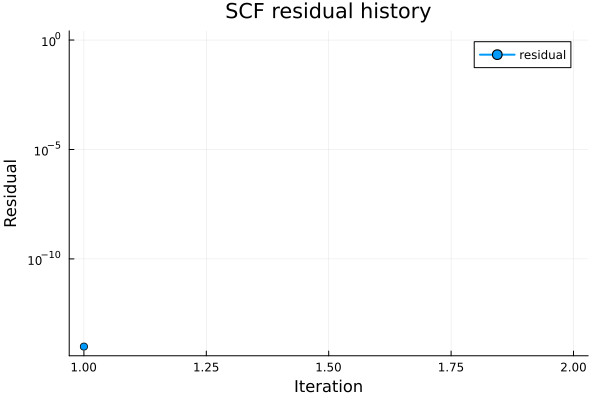
\includegraphics[width=\linewidth]{../../results_vault/experiment_01/OBC/scf_residual.png}

\end{minipage}\hfill%
\begin{minipage}{0.49\linewidth}\centering

\textbf{PBC：収束}\par

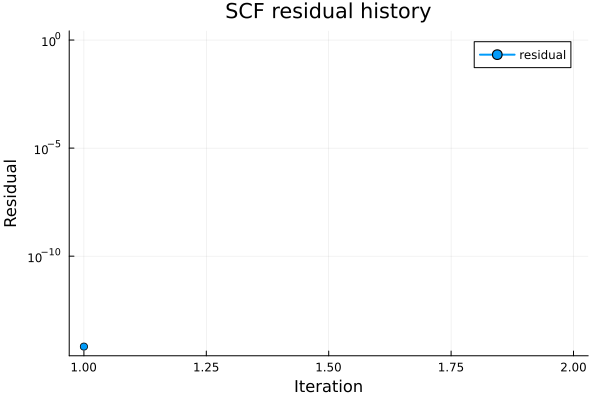
\includegraphics[width=\linewidth]{../../results_vault/experiment_01/PBC/scf_residual.png}

\end{minipage}

\caption{基準条件。SCF残差の比較。左：OBC、右：PBC。}\end{figure}

\chapter{軌道エネルギー：準位構造}

\sourcefile{final_orbital_energies.png}

上下スピンの固有値は重なり、PBCでは波数 $k$ と $-k$ に対応する縮退が階段状に見える。OBCでは $\varepsilon_j=-2t\cos[\pi j/(L+1)]$、PBCでは $\varepsilon_j=-2t\cos(2\pi j/L)$ である。各スピンの低い25準位を足した全エネルギーはログと $10^{-12}$ 未満で一致した。25番目と26番目の準位差はOBCで0.123180、PBCで0.251162であり、相互作用によるギャップではなく有限サイズの準位間隔である。

横軸はエネルギー昇順の軌道番号、縦軸は $h_\sigma=h_0+U\operatorname{diag}(n_{\bar\sigma})$ の固有値である。固有値の数値ファイルは保存されていないため、図からの解釈は定性的なものに留める。未収束例をCSVから再対角化すると保存図とは異なる平均場になる可能性があり、本書ではその置換を行わない。

\begin{figure}[H]\centering

\begin{minipage}{0.49\linewidth}\centering

\textbf{OBC：収束}\par

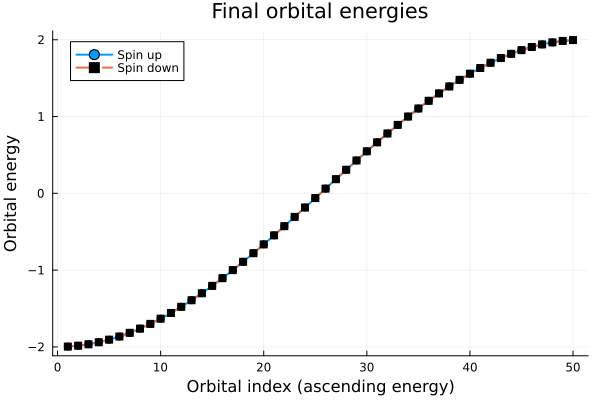
\includegraphics[width=\linewidth]{../../results_vault/experiment_01/OBC/final_orbital_energies.png}

\end{minipage}\hfill%
\begin{minipage}{0.49\linewidth}\centering

\textbf{PBC：収束}\par

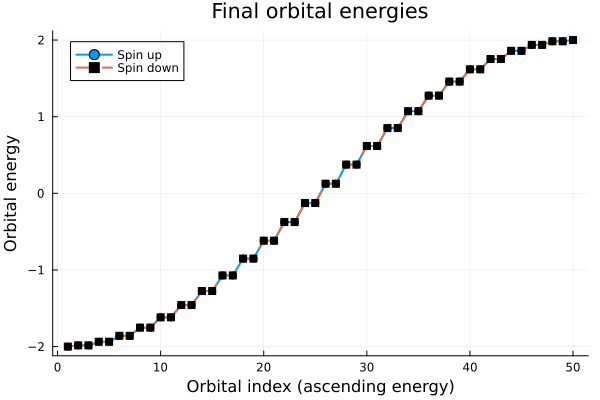
\includegraphics[width=\linewidth]{../../results_vault/experiment_01/PBC/final_orbital_energies.png}

\end{minipage}

\caption{基準条件。軌道エネルギーの比較。左：OBC、右：PBC。}\end{figure}

\chapter{局所磁化：空間構造}

\sourcefile{final_magnetization.png}

全サイトで $m_i=0$ であり、反強磁性も一様なスピン偏極も生じていない。図の縦軸に幅があることは磁化の変動を意味しない。境界条件はエネルギーと準位構造を変えるが、この条件の磁化は変えない。

$\overline{|m|}=L^{-1}\sum_i|m_i|$、$M_{\rm AF}=|L^{-1}\sum_i(-1)^im_i|$ と定義する。$m_i$ はスピン密度差であり、$\langle S_i^z\rangle=m_i/2$ に対応する。全磁化は $\sum_i m_i=\Delta N$ と粒子数制約で固定される。

\begin{center}\small\setlength{\tabcolsep}{4pt}
\begin{longtable}{lrrr}
\toprule
条件/境界 & 状態 & $\overline{|m|}$ & $M_{\rm AF}$ \\ \midrule
\endhead
OBC & 収束 & 0.000000 & 0.000000 \\
PBC & 収束 & 0.000000 & 0.000000 \\
\bottomrule\end{longtable}\end{center}

\begin{figure}[H]\centering

\begin{minipage}{0.49\linewidth}\centering

\textbf{OBC：収束}\par

\includegraphics[width=\linewidth]{../../results_vault/experiment_01/OBC/final_magnetization.png}

\end{minipage}\hfill%
\begin{minipage}{0.49\linewidth}\centering

\textbf{PBC：収束}\par

\includegraphics[width=\linewidth]{../../results_vault/experiment_01/PBC/final_magnetization.png}

\end{minipage}

\caption{基準条件。局所磁化の比較。左：OBC、右：PBC。}\end{figure}

\chapter{境界条件による全エネルギー差}

\sourcefile{boundary_energy_difference.png}

$\Delta E_{\rm boundary}=E_{\rm PBC}-E_{\rm OBC}$ と定義する。負ならPBC、正ならOBCの保存された解の方が低エネルギーである。両方が収束した組だけを表と図で数値比較し、それ以外をNCとする。

差は負で、PBCの方が低エネルギーである。1サイト当たりの差は $-0.015167997582$ である。ただし $L=50$ の1点のみなので、熱力学極限での差の消失やサイズ依存則は本結果だけでは検証できない。

\begin{center}\small\setlength{\tabcolsep}{4pt}
\begin{longtable}{lrr}
\toprule
条件 & $\Delta E_{\rm boundary}$ & $\Delta E_{\rm boundary}/L$ \\ \midrule
\endhead
基準 & -0.758399879117 & -0.015167997582 \\
\bottomrule\end{longtable}\end{center}

\begin{figure}[H]\centering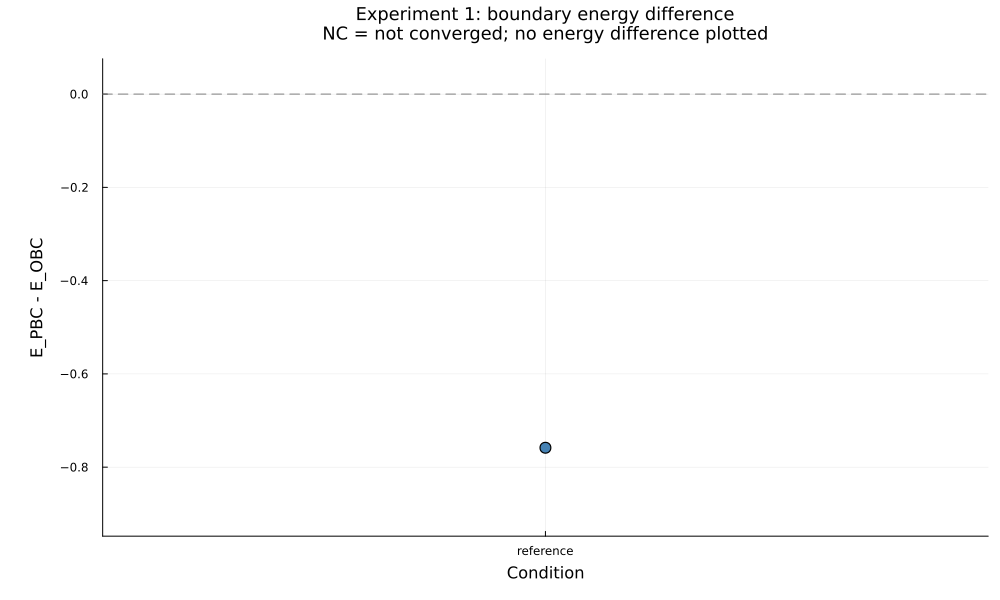
\includegraphics[width=0.9\linewidth]{../../results_vault/experiment_01/boundary_energy_difference.png}\caption{保存済みの境界エネルギー差。NCは未収束の組を示し、差が0であることを意味しない。}\end{figure}

\section*{結論と残された確認}

相互作用を除いた $U=0$ の半充填系を用いて、粒子数、エネルギー、スピン対称性を検算する。両境界条件とも1反復で収束した。$E_{\rm int}=0$ であり、全エネルギーは運動エネルギーと一致する。本実験で変えたのは境界条件だけであり、$U$ や粒子数に関する掃引は行っていない。

対象ケースはすべて収束した。ただし、収束判定だけでは得られた解が大域的な最小エネルギー状態であることまでは保証されない。

サイズは50に固定しているため、境界効果と有限サイズ効果の切り分けには別サイズの結果が必要である。

\end{document}